\subsubsection{Случай Эйлера}
Это простейший частный случай, в котором система динамических уравнений Эйлера интегрируема. Случай Эйлера определяется условием $\vec{M}_A = 0$, это движение тела по инерции.\\

\underline{Интеграл энергии}\\
В силу теоремы об изменении кинетического момента, в случае Эйлера $\vec{K}_A = const$. В силу теоремы об изменении кинетической энергии $T = const$. Тогда получим \textbf{первые интегралы}
\[
K^2 = A^2p^2 + B^2q^2 + C^2r^2 = const
\]
\[
2T = Ap^2 + Bq^2 + Cr^2 = const
\]


\underline{Движение динамически симметричного тела}\\
Пусть выполнено $A = B \neq C$. Заметим, что
\[
\begin{cases}
    \vec{\omega} = p\vec{x} + q\vec{y} + r\vec{z}\\
    \vec{K_A} = Ap\vec{x} + Aq\vec{y} + Cr\vec{z} = A\vec{\omega} + (C - A)r\vec{z}\\
\end{cases} \ \Longrightarrow \vec{\omega} = \dfrac{\vec{K}_A}{A} + \dfrac{A - C}{A}r\vec{z} = \vec{\omega}_1 + \vec{\omega}_2
\]
Т.к. $\vec{K}_A = const$, $\vec{\omega}_1$ постоянна по величине и направлению. Рассмотрим третье из уравнений Эйлера. Т.к. А = В
\[
C\dot{r} = 0 \Longrightarrow r = const
\]
Значит, $\vec{\omega}_2$ постоянна по величине. А т.к. $K^z = \vec{K}\cdot\vec{z} = Cr = K\cos{\Theta} = const$, угол между двумя компонентами угловой скорости тоже не меняется. Таким образом, имеет место регулярная прецессия (причем свободная, т.к. момент внешних сил равен нулю) с параметрами
\[
\dot{\psi} = \omega_1 = \dfrac{K}{A} \tab \dot{\phi} = \omega_2 = \dfrac{A - C}{A}r \tab \cos{\Theta} =\dfrac{Cr}{K}
\]
Они связаны соотношением
\[
C\omega_2 + (C - A)\omega_1 \cos{\Theta} = 0
\]

Еще один простой случай: $A = B = C$. Не будем рассматривать его подробно, скажем лишь, что тут получится, что $\vec{\omega} = const$, а движение --- это вращение с постоянной скоростью вокруг неподвижной оси.\\

Перейдем к общему случаю. Для определенности положим, что $A > B> C$. Пусть $a,~b,~c$ и $d$ --- параметры, которые однозначно выражаются через исходные параметры задачи из интегралов энергии. Тогда $p$ и $r$ выражаются как
\[
p = \pm \sqrt{a - bq^2}, \tab r = \pm \sqrt{c - dq^2}\eqno{(*)}
\]
Подставим эти выражения во второе из уравнений Эйлера:
\[
B\dot{q} \pm (A - C)\sqrt{(a - bq^2)(c - dq^2)} = 0
\]
Отсюда можно найти $q(t)$ обращением эллиптического интеграла
\[
\int\limits_0^q \dfrac{dq}{\sqrt{(a - bq^2)(c - dq^2)}} = \pm \dfrac{C - A}{B}(t - t_0)
\]

\begin{frame}{Прим. редактора}
    Обращение делается при помощи эллиптических функций, которые мы не будем сейчас подробно рассматривать. Почитать про них можно \href{https://ru.wikipedia.org/wiki/%D0%AD%D0%BB%D0%BB%D0%B8%D0%BF%D1%82%D0%B8%D1%87%D0%B5%D1%81%D0%BA%D0%B0%D1%8F_%D1%84%D1%83%D0%BD%D0%BA%D1%86%D0%B8%D1%8F}{здесь (кратко)} и \href{https://staff.math.su.se/mleites/books/prasolov-soloviev-1997-elliptic.pdf}{здесь (книга)}.\\
\end{frame}

Тогда с помощью $(*)$ сможем определить $p(t)$ и $r(t)$. Таким образом, динамические уравнения в случае Эйлера интегрируются независимо от кинематических.\\

Для того, чтобы показать, что в случае Эйлера уравнения вращательного движения интегрируются при любых начальных условиях, осталось доказать, что при такой постановке задачи с известными зависимостями $p(t)$, $q(t)$ и $r(t)$ интегрируются кинематические уравнения в углах Эйлера.\\

\begin{minipage}{0.6\textwidth}
    Вернемся к рассмотрению тела в инерциальном базисе $O_{xyz}$ таком, что $\vec{z}$ направлен вдоль вектора кинетического момента. Тогда его проекции на оси
    \[
    \begin{cases}
        K^x = Ap = K\sin{\Theta}\sin{\phi}\\
        K^y = Bq = K\sin{\Theta} \cos{\phi}\\
        K^z = Cr = K\cos{\Theta}\\
    \end{cases}
    \]
    Отсюда находим
    \end{minipage}
    \hfill%
\begin{minipage}{0.3\textwidth}\raggedright% adapt widths of minipages to your needs
    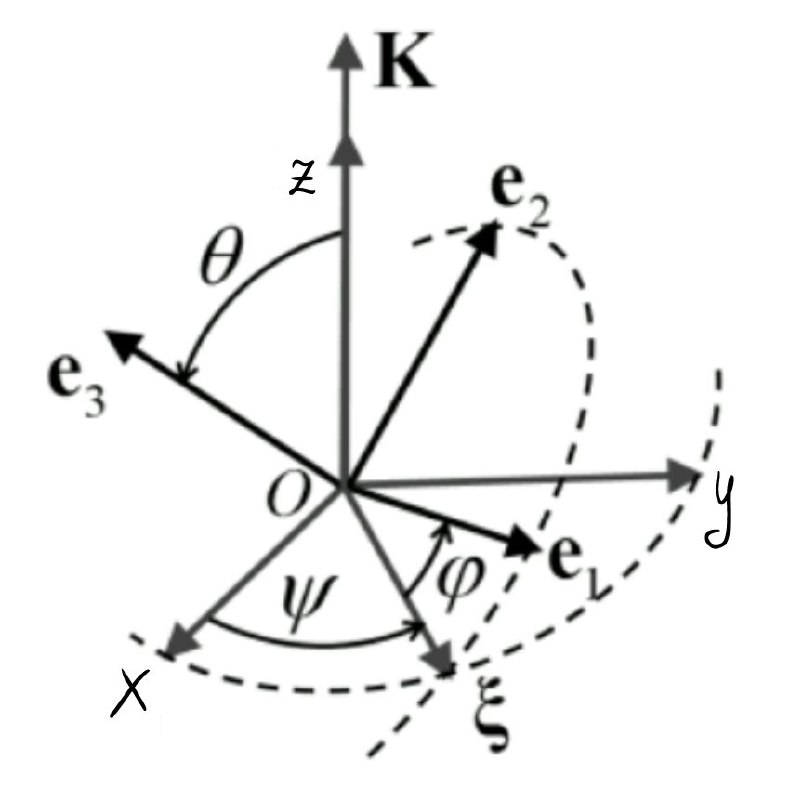
\includegraphics[width=1.0\textwidth]{images/лекция_9_1.jpeg} 
\end{minipage}%    

\[
\cos{\Theta} = \dfrac{Cr(t)}{K}, \tab \cos{\phi} = \dfrac{Bq(t)}{K\sin{\sin{\Theta}}}
\]
Угол прецессии найдем интегрированием первого из кинематических уравнений Эйлера:
\[
\psi(t) = \psi(0) + \int\limits_0^t\dfrac{p(t)\sin{\phi(t)} + q(t)\cos{\phi(t)}}{\sin{\Theta(t)}}dt
\]
Получили требуемое.\\

Аналитические решения полученных уравнений слишком сложны и не являются наглядными, поэтому используются геометрические интерпретации.\\

\underline{Геометрическая интерпретация Мак-Куллага}\\
\begin{figure}[!h]
    \centering
    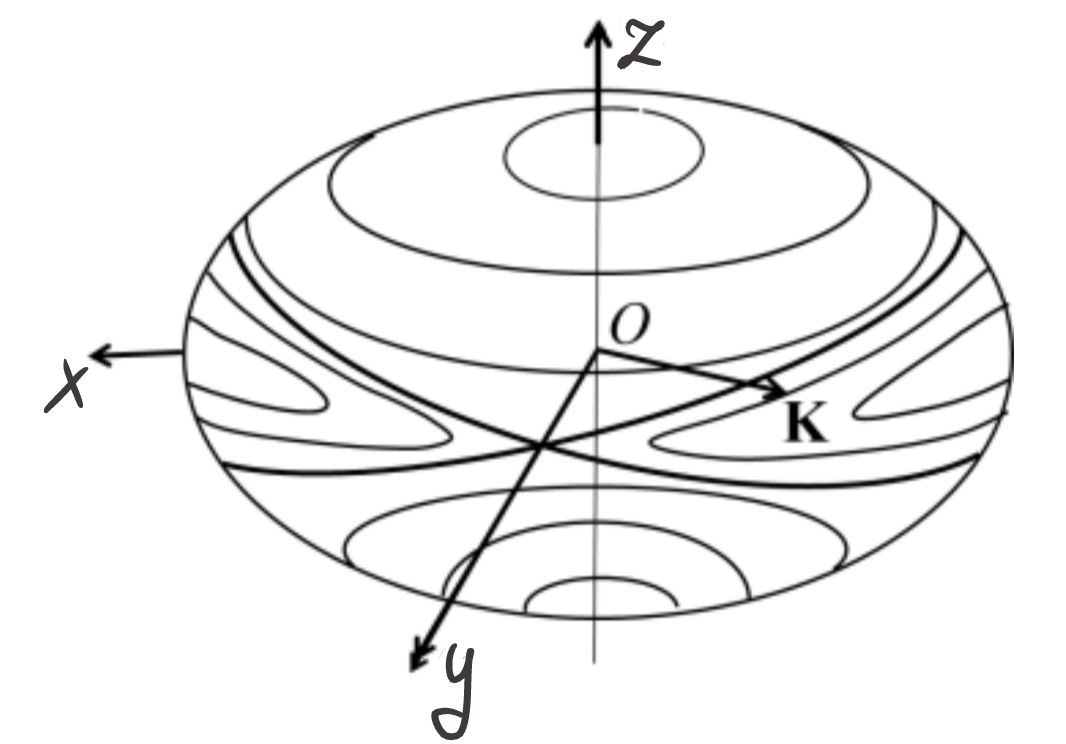
\includegraphics[width=0.5\linewidth]{images/лекция_9_2.jpeg}
\end{figure}

    Используя интегралы энергии, получим:
    \[
    (K^x)^2 + (K^y)^2 + (K^z)^2 = K^2
    \]
    \[
    \dfrac{(K^x)^2}{A} + \dfrac{(K^y)^2}{B} + \dfrac{(K^z)^2}{C} = 2T
    \]
    В осях $(K^x,~K^y,~K^z)$ первое уравнение представляет собой сферу с радиусом $K$, а второе --- \textbf{эллипсоид Мак-Куллага} (или Мак-Куллаха) с полуосями $\sqrt{2TA}$, $\sqrt{2TB}$ и $\sqrt{2TC}$. В процессе движения вектор кинетического момента должен принадлежать пересечению этих поверхностей (это возможно, если $2TA \geq K^2 \geq 2TC$), при этом линии пересечения --- это траектории этого вектора на поверхности эллипсоида Мак-Куллага, неподвижного в теле.\\

Если в какой-то момент времени вектор $\vec{K}$ близок по направлению к оси среднего момента инерции $\vec{y}$, то в дальнейшем, двигаясь по соответствующей траектории, он в какой-то момент времени займет на поверхности эллипсоида Мак-Куллага положение, близкое по направлению к оси $-\vec{y}$. Это означает, что по отношению к неподвижному в инерциальном базисе вектору кинетического момента ось $\vec{y}$ поменяет свое направление на обратное.\\

Если учесть еще, что скорость вектора кинетического момента относительно тела $\dot{\vec{K}}^\text{отн} = \vec{K}\times J^{-1}\times{\vec{K}}$ и она тем меньше, чем ближе вектор $\vec{K}$
по направлению к оси $\vec{y}$ или $-\vec{y}$, то этого будет достаточно для объяснения эффекта Джанибекова, в котором закрученное вокруг оси среднего момента инерции тело неоднократно и почти скачкообразно меняет направление этой оси в пространстве на обратное.\\

\begin{frame}{Прим. редактора}
    Демонстрация \href{https://www.youtube.com/watch?v=L2o9eBl_Gzw}{эффекта Джанибекова}.\\
\end{frame}

\underline{Геометрическая интерпретация Пуансо}\\
В этой интерпретации движение тела описывается движением связанного с ним эллипсоида инерции. В случае Эйлера эллипсоид инерции катится без проскальзывания по неподвижной плоскости, ортогональной вектору кинетического момента.\\
\begin{proof}
    Напомним, что с помощью тензора инерции и угловой скорости можно получить соотношения $\vec{K} = J\vec{\omega}$ и $T = \dfrac{1}{2} = \vec{\omega}^TJ\vec{\omega}$. Уравнение эллипсоида
    \[
    f = \vec{r}^TJ\vec{r} - 1 = 0
    \]
    Пусть $P$ ($\vec{r}_P = r_P\dfrac{\vec{\omega}}{\omega}$) --- неподвижная точка на поверхности эллипсоида. Проведем через нее ортогонально $\vec{K}$ плоскость П. Из уравнения эллипсоида
    \[
    \dfrac{r_P^2}{\omega^2} = \dfrac{1}{2T}
    \]
    Нормаль к поверхности в точке $P$
    \[
    \vec{\eta} = \dfrac{\partial f}{\partial \vec{r}}\mid_P = 2J\vec{r}\mid_P = \dfrac{2r_P}{\omega}\vec{K}
    \]
    $\Longrightarrow$ в точке $P$ эллипсоид инерции касается плоскости П.\\

    Расстояние от центра эллипсоида до П
    \[
    h = \dfrac{\vec{r}_P^T\vec{K}}{K} = \dfrac{\sqrt{2T}}{K}
    \]
    Причем $h = const$ в случае Эйлера, т.к. $T = const$ и $K = const$.
\end{proof}

\begin{frame}{Прим. редактора}
    Демонстрация геометрической интерпретации \href{https://www.youtube.com/watch?v=BwYFT3T5uIw}{Пуансо}.
\end{frame}
